\chapter*{\allyId}

\label{site}

\begin{paracol}{2}
\begin{leftcolumn}
We promise ourselves that we live our memories in a linear fashion. And who knows, perhaps we do.

What we emphatically do not do is remember our lives in linear fashion. \allyWord\ began as an interactive project specifically to explore this aspect. The goal was to use the concept of interlinked pages to represent the way that one memory can be interlinked to another, and another, and so on.

\begin{ally}
  And dreadfully distinct within the dark, a tall white fountain played?
\end{ally}
Something like that.

And here, we lean on a very specific deinition of hypertext. Hypertext is used to imply that some portion of a document can link to another portion of a document. This linking goes beyond simply the links that one clicks, as it can mean inclusions, such as when an image is included on a page full of text. It can, indeed, mean a link that leads from one page to the next, but what means `next' here? Does it mean moving on to the next page in a series of pages, or does it mean moving from one section of the site to another? Perhaps it means moving from this site to the next.

\end{leftcolumn}
\begin{rightcolumn*}
\newpage
\section*{Hypertext types}
\begin{labeling}{Arborescent}
  \item[Axial] A set of linked documents that travels down a single axis, from start to finish.
  \item[Arborescent] A set of linked documents with a central axis, of of which may sprout other documents (which may in turn be axial or arborescent hypertexts).
  \item[Networked] A set of linked documents with no discernable axis. No start or finish, no direction to travel in.
\end{labeling}
\end{rightcolumn*}
\begin{leftcolumn}

With \allyId, this became a core component of exploring memory. It means something different to wind one's way down the singular path a memory treads than it does to jump the track onto something wholly different. The central axis of the story is the death of Matthew as told through conversations with--

\begin{ally}
  Me!
\end{ally}
--with an imaginary alter-ego who, by virtue of that `ego', knows all the same things I do.

\begin{ally}
  Or more.
\end{ally}
Perhaps, yes.

As a memory would be touched upon, it would spark a new branch of exploration that would proceed in much the same way. This is why the project is described as ``arborescent'': there is a central trunk with a defined beginning at the root, and from there, it blossoms up and out.

Or, it turns out, down and out.
\newpage

\end{leftcolumn}
\begin{rightcolumn*}
\begin{verse}
\begin{spacing}{-10}
{\MonoFont
.\\
├── about.md\\
├── ally\\
│   ├── 001.md\\
│   ├── 002.md\\
│   ├── ...\\
│   └── \_index.md\\
├── birds\\
│   ├── 01.md\\
│   ├── 02.md\\
│   ├── ...\\
│   └── \_index.md\\
├── burnout\\
│   ├── 01.md\\
│   ├── 02.md\\
│   ├── ...\\
│   └── \_index.md\\
├── dad\\
│   ├── 001.md\\
│   ├── 002.md\\
│   ├── ...\\
│   ├── as\\
│   │   └── a\\
│   │       └── person\\
│   │           ├── 001.md\\
│   │           ├── 002.md\\
│   │           ├── 003.md\\
│   │           ├── 004.md\\
│   │           ├── 005.md\\
│   │           └── \_index.md\\
│   └── \_index.md\\
└── ...
}
\end{spacing}
\end{verse}

\end{rightcolumn*}
\begin{leftcolumn}
\noindent While working on \allyId, Each page was kept in a single Markdown file, and each exploring branch was kept in a folder. Thus, we wind up with a file structure akin to what we see on the right.

\begin{ally}
  Never content to condense your thoughts into something simple and easy to read, were you?
\end{ally}
To your scattered files go, I suppose.

Do keep in mind that this is a website, however. This directory, these filenames, this structure all play a role in how the whole project works. These whole tree of files are in the \texttt{content} directory of a Hugo project. Hugo is a program which knows how to take these Markdown files and turn them into HTML files while following a simple set of rules.

In each of those \texttt{\_index.md} files, one will usually find nothing. That is, in terms of content, for at the top of each file comes a header which describes some of those rules. For instance, in some directories, we want the background to be a certain color, or perhaps we want there to be a link down at the bottom saying ``back to where we left off''.

\begin{ally}
  There is no going, and there is no back.
\end{ally}
We can always pretend.

Another rule that is stated in these files is that they are intended to list the pages in that directory. Usually, this is done on a blog page where you might see the titles and first paragraphs of ten blog entries in a list, each with a ``read more'' link, followed at the bottom by a list of `pages of results'. In my case, though, I set Hugo up so that, when it listed all of the `posts', it would only do one per page, and instead of showing only the first paragraph, it would show the whole page. This essentially made it work as a book would: you simply turn the page when you're done reading. My \texttt{list.html} file for this `serial' layout loops over the pages in the directory as follows:

\begin{verbatim}
{{ $paginator := .Paginate .Pages.ByWeight 1 }}
{{ $content := .Content }}
{{ range $paginator.Pages.ByWeight }}
...
\end{verbatim}

With this theme in place and with the files all in the right orders (each with a \texttt{weight} key in their own headers), Hugo will build the site as it stands.

\begin{ally}
  Oh, but there's more to it than that.
\end{ally}
Of course.

\newpage
\end{leftcolumn}
\begin{rightcolumn*}
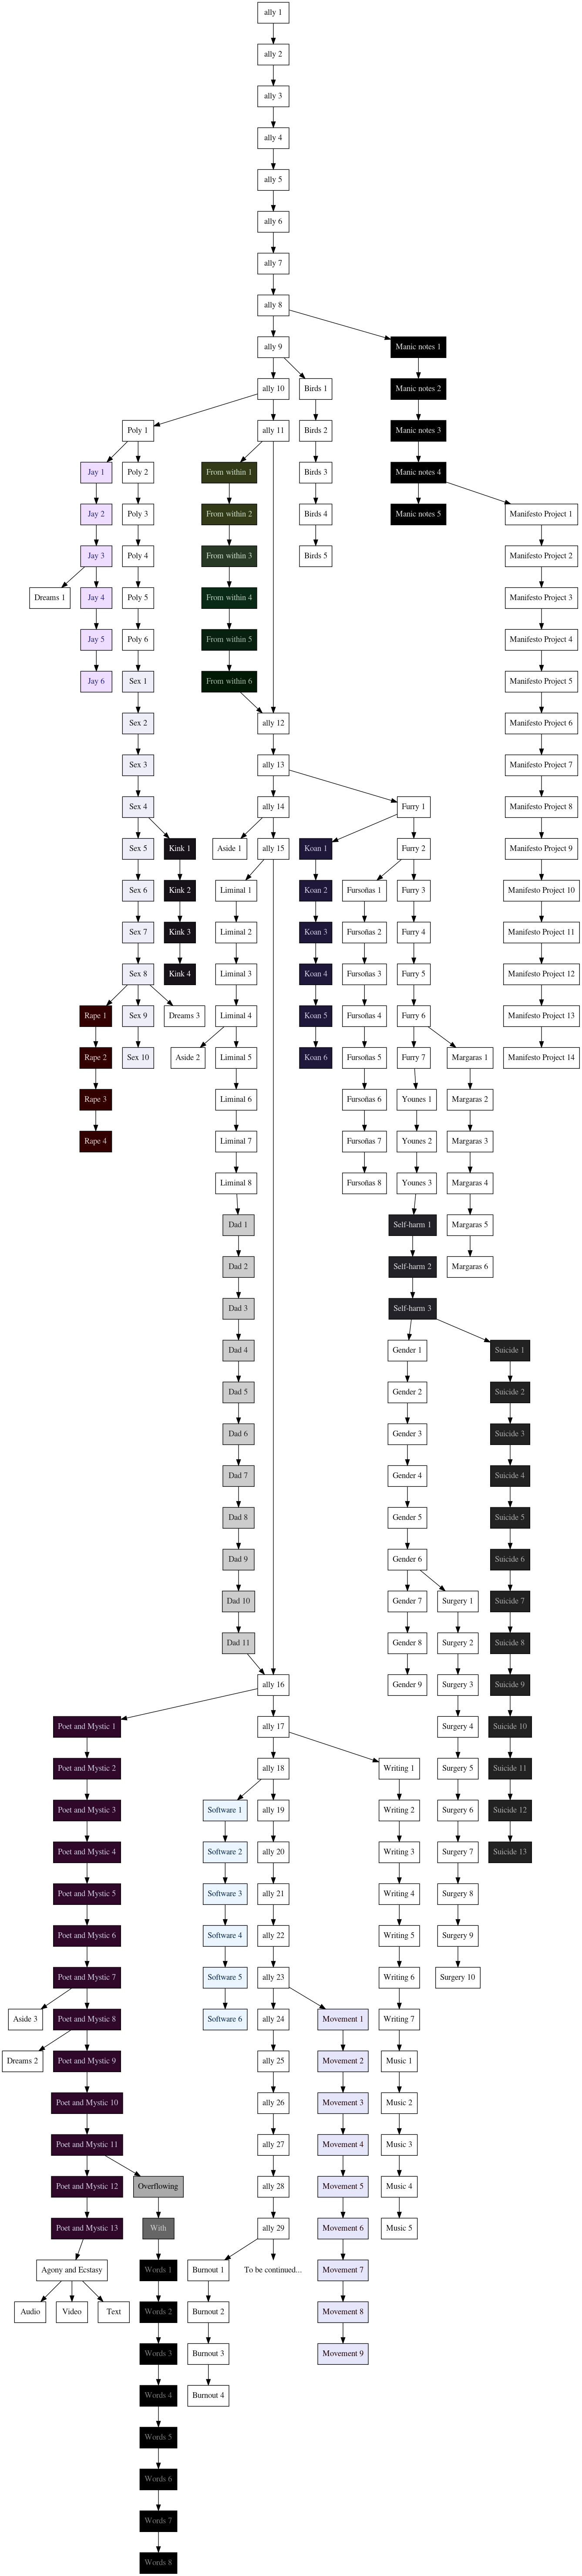
\includegraphics[width=2.5in]{assets/map.png}
\end{rightcolumn*}
\begin{leftcolumn}

\noindent Early on in \allyId's life, I decided that there needed to be a map of the site. A literal map, too. No carefully broken down list of links for you to click on, but something more clearly representing the paths one takes through memory.

\begin{ally}
  Your ``Catastrophically Maddy'' counter is ticking up.
\end{ally}
Did you expect anything less?

\begin{ally}
  I suppose not. Carry on.
\end{ally}
Score one for Maddy.

So, even thought it takes a bit of work by hand everytime I add a page, I decided that it would be worth it to construct a graph that showed the arborescent nature of the project. I was tempted at one point to do the whole thing in Javascript using SVG so that it would track your movement through the pages, but even that was too much for me.

\begin{ally}
  Wonder of wonders.
\end{ally}
So instead, I leveraged existing tools--

\begin{ally}
  Gag.
\end{ally}
Right, sorry. So instead, I decided to use what I already had installed, which meant dusting off my knowledge of Graphviz.

In my \texttt{assets} folder lives a \texttt{map.dot} file which contains a node for every page and the edges that connect them. It's easy to add to; every time I add a new branch, I list every page inside of it along with its URL, and then draw all of the links that connect those pages together. At the bottom, there is the links from the trunk (or parent branch) to the branches.

\begin{verbatim}
digraph Map {
    node[group="dad",
         style="filled",
         fillcolor="#cccccc",
         fontcolor="#222222"]
    "Dad 1" [href="/dad"]
    "Dad 2" [href="/dad/2"]
    "Dad 3" [href="/dad/3"]
    "Dad 4" [href="/dad/4"]
    "Dad 5" [href="/dad/5"]
    "Dad 6" [href="/dad/6"]
    "Dad 7" [href="/dad/7"]
    "Dad 8" [href="/dad/8"]
    "Dad 9" [href="/dad/9"]
    "Dad 10" [href="/dad/10"]
    "Dad 11" [href="/dad/11"]
    "Dad 1" -> "Dad 2" -> "Dad 3" -> "Dad 4" -> "Dad 5" ->
    "Dad 6" -> "Dad 7" -> "Dad 8" -> "Dad 9" -> "Dad 10" ->
    "Dad 11"
\end{verbatim}

And so on, until:

\begin{verbatim}
    "ally 29" -> "Burnout 1"
    "As a person 5" -> "ally 16"
    "From within 6" -> "ally 12"
    "Younes 3" -> "Self-harm 1"
    "Furry 1" -> "Koan 1"
    "Jay 3" -> "Dreams 1"
    "Liminal 8" -> "Dad 1"
}
\end{verbatim}
\newpage

While the whole file is much, much larger than just this, it is really no more complicated\footnote{Except\ldots{} --- page \pageref{branchdir}}. I rarely go back and change orders, and almost never tack a branch onto the trunk in a different place, so I just trace the lines once and let Graphviz sort the rest out.

Once I've updated the Dot file with the new pages, I type \texttt{make}, which, on seeing that the file has changed, runs \texttt{dot -Tsvg map.dot -omap.svg}, which generages the image itself.

The cool part about SVG is that it renders in the browser just as well as HTML, including with clickable links, so I get a \emph{navigable} sitemap for free. All I need to do is copy and paste the contents of that \texttt{map.svg} file into the proper place in the site\footnote{\ldots{}sorta --- page \pageref{svgfont}}. 

\newpage

We have our content, we have our map, now we just need a way to get it up on the web so that others can see it, right?

\begin{ally}
  A question like that never has an easy answer.
\end{ally}
Correct.

Hugo generates a set of folders filled with HTML files and static assets. It's no good on my machine, since that'd mean that I'm the only one that can see it. I could FTP the project up to a server and drop it where everyone could see that but\ldots{}you know, now that I think about it, I can't remember the last time I used FTP.

Better, instead to just have another tool do it for me. Two other tools, actually.

\begin{ally}
  You know, if you are trying to sell this as an easy way to approach a project, I don't know that you are succeeding.
\end{ally}
This is fair. One of the reasons it feels easy to me is that I was already running several other projects using the same technology. The reasons those work so well for me are closely tied with how I run my writing setup, and how I use my writing setup is closely tied with how I program.

It makes sense for me to have a system that relies on convention over configuration, given how many software projects have worked that way. It makes sense for me to have a system that relies on publishing stories in files rather than database entries as I might with Wordpress or Ghost, given how much of my life is spent tooling around with other files. I'm hardly recommending this as a path forward. There are doubtless easier ways, regardless of how well this worked for me.

\begin{ally}
  Right.
\end{ally}
Right.

So, given this Hugo site, the best way for me to work with deploying it uses a pair of tools: Github, which allows me to keep the entire site in a version-controlled repository synced remotely, and Netlify which will automatically build and serve static sites such as this one.
\end{leftcolumn}
\begin{rightcolumn*}
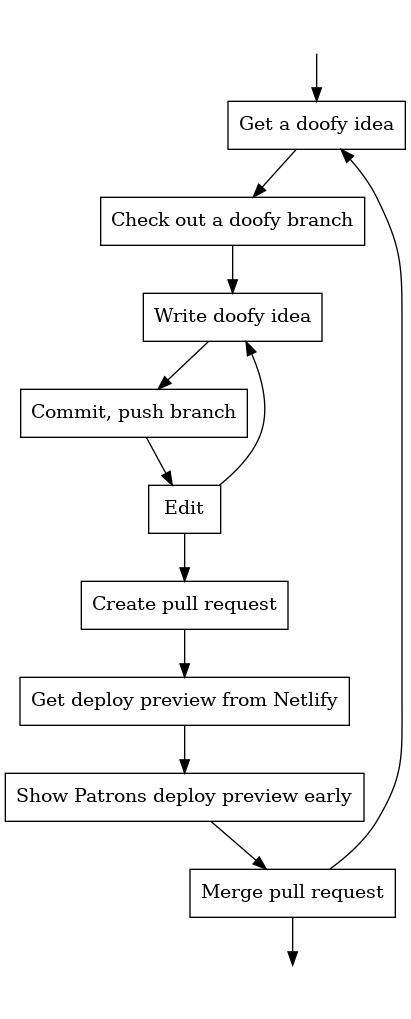
\includegraphics[width=2in]{assets/workflow.png}
\end{rightcolumn*}
\begin{leftcolumn}

When I get an idea for a ``sidequest'' to work on with \allyWord, I create a branch away from the \texttt{master} branch --- `branch' both in terms of git as well as in terms of hypertext, here --- and work there. When I push that branch up to Github and create a pull request, Netlify sees this and automatically creates a deploy preview which I can share with those Patrons who get early access. When I click the big grean ``merge'' button on github, Netlify then builds the main site which everyone can see
\newpage
\end{leftcolumn}
\end{paracol}
